\documentclass[../poma-notes.tex]{subfiles}

\graphicspath{\subfix{../images/}}

\begin{document}

\subsection*{Finite, Countable, and Uncoutable Sets}

本节由函数概念的定义开始。

\begin{definition}
  Consider two sets $A$ and $B$, whose elements may be any objects whatsover, and suppose that with each
  element $x$ of $A$ there is associated, in some manner, an element of $B$, which we denote by $f(x)$.
  Then $f$ is said to be a \textit{function} from $A$ to $B$ (or a \textit{mapping} of $A$ into $B$).
  The set $A$ is called the \textit{domain} of $f$ (we also say $f$ is defined on $A$), and the elements $f(x)$
  are called the \textit{values} of $f$. The set of all values of $f$ is called the \textit{range} of $f$.
\end{definition}

\begin{definition}
  Let $A$ and $B$ be two sets and let $f$ be a mapping of $A$ into $B$. If $E \subset A$, $f(E)$ is defined to
  be the set of all elements $f(x)$, for $x \in E$. We call $f(E)$ the \textit{image} of $E$ under $f$.
  In this notation, $f(A)$ is the range of $f$. It is clear that $f(A) \subset B$. If $f(A)=B$, we say that $f$
  maps $A$ \textit{onto} $B$. (Note that, according to this usage, \textit{onto} is more specific than \textit{into}.)

  If $E \subset B$, $f^{-1}(E)$ denotes the set of all $x \in A$ such that $f(x) \in E$. We call $f^{-1}(E)$ the
  \textit{inverse image} of $E$ under $f$. If $y \in B$, $f^{-1}(y)$ is the set of all $x \in A$ such that
  $f(x)=y$. If, for each $y \in B$, $f^{-1}(y)$ consists of at most one element of $A$, then $f$ is said to be
  a 1-1 (\textit{one-to-one}) mapping of $A$ into $B$. This may also be expressed as follows: $f$ is a 1-1 mapping
  of $A$ into $B$ provided that $f(x_1) \ne f(x_2)$ whenever $x_1 \ne x_2,\ x_1 \in A,\ x_2 \in A$.

  (The notation $x_1 \ne x_2$ means that $x_1$ and $x_2$ are distinct elements; otherwise we write $x_1=x_2$.)
\end{definition}

\begin{anote}
  简单来说:
  \begin{enumerate}
    \item $f(E)$ 是集合 $E$ 通过 $f$ 得到的像(image)。
    \item $f(A)$ 是 $f$ 的范围。
    \item 如果 $f(A)=B$,那么称 $f$ 将 $A$ 完全映射至(onto)$B$ 。
    \item 而当 $E \subset B$ 且 $x \in A$ 时,反函数 $f^{-1}(E)$ 是集合 $E$ 通过 $f$ 得到的反像(inverse image)。
    \item $\forall x \in A$ 通过 $f$ 映射后且满足 $\forall f(x) \in B$ 被称为一一映射(1-1 mapping)。
  \end{enumerate}
\end{anote}

\begin{definition}
  If there exists a 1-1 mapping of $A$ \textit{onto} $B$, we say that $A$ and $B$ can be put in 1-1 \textit{correspondence},
  or that $A$ and $B$ have the same \textit{cardinal number}, or, briefly, that $A$ and $B$ are \textit{equivalent},
  and we write $A \sim B$. This relation clearly has the following properties:
  \begin{itemize}
    \item[] It is reflexive: $A \sim A$.
    \item[] It is symmetric: If $A \sim B$, then $B \sim A$.
    \item[] It is transitive: If $A \sim B$ and $B \sim C$, then $A \sim C$.
  \end{itemize}
  Any relation with these three properties is called an \textit{equivalence relation}.
\end{definition}

\anote Reflexive 自反性,\href{https://en.wikipedia.org/wiki/Reflexive_relation}{维基百科}。

\begin{definition}
  For any positive integer $n$, let $J_n$ be the set whose elements are the integers $1,2,\dots,n$; let $J$ be
  the set consisting of all positive integers. For any set $A$, we say:
  \begin{enumerate}[label=(\alph*)]
    \item $A$ is \textit{finite} if $A \sim J_n$ for some $n$ (the empty set is also considered to be finnite).
    \item $A$ is \textit{infinite} if $A$ is not finite.
    \item $A$ is \textit{countable} if $A \sim J$.
    \item $A$ is \textit{uncountable} if $A$ is neither finite nor countable.
    \item $A$ is \textit{at most countable} if $A$ is finite or countable.
  \end{enumerate}

  Countable sets are sometimes called \textit{enumerable}, or \textit{denumerable}.

  For two finite sets $A$ and $B$, we evidently have $A \sim B$ if and only if $A$ and $B$ contain the same number of
  elements. For infinite sets, however, the idea of \say{having the same number of elements} becomes quite vague,
  whereas the notion of 1-1 correspondence retains its clarity.
\end{definition}

\anote
可数集(countable set),是指每个元素都能与自然数集 $N$ 的每个元素之间能建立一一对应的集合;不可数集顾名思义就是无法与自然数集
$N$ 建立一一对应的集合;至多可数集(at most coutable)是有限集(finite)与可数集(coutable)的统称。

\setcounter{poma}{6}

\begin{definition}
  By a \textit{sequence}, we mean a function $f$ defined on the set $J$ of all positive integers. If $f(n)=x_n$,
  for $n \in J$, it is customary to denote the sequence $f$ by the symbol $\{x_n\}$, or sometimes by $x_1,x_2,x_3,\dots$.
  The values of $f$, that is, the elements $x_n$, are called the \textit{terms} of the sequence. If $A$ is a set and
  if $x_n \in A$ for all $n \in J$, then $\{x_n\}$ is said to be a \textit{sequence} in $A$, or a \textit{sequnce of elements}
  of $A$.
\end{definition}

注意一个数列的 $x_1,x_2,x_3,\dots$ 项不需要是独特的。

由于每个可数集合是一个定义在 $J$ 上一一映射的范围,可将每个可数集合视为一系列不同项的范围。更宽泛来说,任何可数集合中的原始可以被
“排列在一个数列上”。

有时可以将定义中的 $J$ 替换为所有非负整数集合,这样可能会更加的方便,例如开始于 0 而不是 1。

\begin{theorem}
  Every infinite subset of a countable set $A$ is coutable.
\end{theorem}

\begin{proof}
  假设 $E \subset A$,且 $E$ 为无限的。排列 $A$ 中的元素 $x$ 构建 $\{x_n\}$ 独特数列。构建一个满足如下的数列 $\{n_k\}$:

  令 $n_1$ 为最小的正整数使得 $x_{n_1} \in E$。选择 $n_1,\dots,n_{k-1} \ (k=2,3,4,\dots)$,令 $n_k$ 为最小的大于 $n_{k-1}$
  的整数使得 $x_{n_k} \in E$。

  令 $f(k)=x_{n_k} \ (k=1,2,3,\dots)$,我们获取一个 $E$ 与 $J$ 的一一映射关系。

  根据定理,粗略的说可数集合表示了\say{最小的}无限性:没有不可数集合可以成为一个可数集合的子集。
\end{proof}

\anote
一个可数集合 $A$ 的任意无限子集都是可数的。

\begin{definition}
  Let $A$ and $\Omega$ be sets, and suppose that with each element $\alpha$ of $A$ there is associated a subset of
  $\Omega$ which we denote by $E_{\alpha}$.

  The set whose elements are the sets $E_{\alpha}$ will be denoted by $\{E_{\alpha}\}$. Instead of speaking of sets
  of sets, we shall sometimes speak of a collection of sets, or a family of sets.

  The \textit{union} of the sets $E_{\alpha}$ is defined to be the set $S$ such that $x \in S$ if and only if
  $x \in E_{\alpha}$ for at least one $\alpha \in A$. We use the notation
  \begin{equation}
    S = \bigcup \limits_{\alpha\in A} E_{\alpha}.
  \end{equation}
  If $A$ consists of the integers $1,2,\dots,n$, one usually writes
  \begin{equation}
    S = \bigcup \limits_{m=1}^n E_m
  \end{equation}
  or
  \begin{equation}
    S = E_1 \cup E_2 \cup \cdots \cup E_n.
  \end{equation}
  If $A$ is the set of all positive integers, the usual notation is
  \begin{equation}
    S = \bigcup \limits_{m=1}^{\infty} E_m.
  \end{equation}

  The symbol $\infty$ in (4) merely indicates that the union of a \textit{countable} collection of sets is taken,
  and should not be confused with the symbols $+\infty$, $-\infty$, introduced in Definition 1.23.

  The \textit{intersection} of the sets $E_{\alpha}$ is defined to be the set $P$ such that $x \in P$ if and only if
  $x \in E_{\alpha}$ for every $\alpha \in A$. We use the notation
  \begin{equation}
    P = \bigcap \limits_{\alpha \in A} E_{\alpha},
  \end{equation}
  or
  \begin{equation}
    P = \bigcap \limits_{m=1}^n E_m = E_1 \cap E_2 \cap \cdots \cap E_n,
  \end{equation}
  or
  \begin{equation}
    P = \bigcap \limits_{m=1}^{\infty} E_m,
  \end{equation}
  as for unions. If $A \cap B$ is not empty, we say that $A$ and $B$ \textit{intersect}; otherwise they are \textit{disjoint}.
\end{definition}

\anote
$S$ 代表所有 $E_{\alpha}$ 集合的并集;$P$ 代表所有 $E_{\alpha}$ 集合的交集。

\refstepcounter{poma}
\begin{remark}
  Many properties of unions and intersections are quite similar to those of sums and products; in fact,
  the words sum and product were sometimes used in this connection, and the symbols $\Sigma$ and $\Pi$
  were written in place of $\bigcup$ and $\bigcap$.

  The commutative and associative laws are trivial:
  \begin{equation}
    A \cup B = B \cup A; \quad A \cap B = B \cap A.
  \end{equation}
  \begin{equation}
    (A \cup B) \cup C = A \cup (B \cup C); \quad (A \cap B) \cap C = A \cap (B \cap C).
  \end{equation}
  Thus the omission of parenthese in (3) and (6) is justified.

  The distributive law also holds:
  \begin{equation}
    A \cap (B \cup C) = (A \cap B) \cup (A \cap C).
  \end{equation}
  To prove this, let the left and right members of (10) be denoted by $E$ and $F$, respectively.

  Suppose $x \in E$. Then $x \in A$ and $x \in B \cup C$, that is, $x \in B$ or $x \in C$ (possibly both).
  Hence $x \in A \cap B$ or $x \in A \cap C$, so that $x \in F$. Thus $E \subset F$.

  Next, suppose $x \in F$. Then $x \in A \cap B$ or $x \in A \cap C$. That is, $x \in A$, and
  $x \in B \cup C$. Hence $x \in A \cap (B \cup C)$, so that $F \subset E$.

  It follows that $E = F$.

  We list a few more relations which are easily verified:
  \begin{equation}
    A \subset A \cup B,
  \end{equation}
  \begin{equation}
    A \cap B \subset A.
  \end{equation}
  If 0 denotes the empty set, then
  \begin{equation}
    A \cup 0 = A, \quad A \cap 0 = 0.
  \end{equation}
  If $A \subset B$, then
  \begin{equation}
    A \cup B = B, \quad A \cap B = A.
  \end{equation}
\end{remark}

\begin{theorem}
  Let $\{E_n\},\ n=1,2,3,\dots$, be a sequence of countable sets, and put
  \begin{equation}
    S = \bigcup \limits_{n=1}^{\infty} E_n.
  \end{equation}
  Then $S$ is countable.
\end{theorem}

\begin{proof}
  Let every set $E_n$ be arranged in a sequence $\{x_{nk}\},\ k=1,2,3,\dots$, and consider the infinite array
  \begin{equation}
    \begin{tikzpicture}[baseline=(current bounding box.center)]
      \matrix[
        matrix of math nodes,
        nodes in empty cells,
      ](m) {
        x_{11} & x_{12} & x_{13} & x_{14} & \dots \\
        x_{21} & x_{22} & x_{23} & x_{24} & \dots \\
        x_{31} & x_{32} & x_{33} & x_{34} & \dots \\
        x_{41} & x_{42} & x_{43} & x_{44} & \dots \\
        \dots  & \dots  & \dots  & \dots  & \dots \\
      };
      \draw [->] (m-1-1.-150) -- (m-1-1.30);
      \draw [->] (m-2-1.-150) -- (m-1-2.30);
      \draw [->] (m-3-1.-150) -- (m-1-3.30);
      \draw [->] (m-4-1.-150) -- (m-1-4.30);
    \end{tikzpicture}
  \end{equation}

  in which the elements of $E_n$ form the $n$th row. The array contains all elements of $S$. As indicated by
  the arrows, these elements can be arranged in a sequence
  \begin{equation}
    x_11;x_21,x_12;x_32,x_22,x_13;x_41,x_32,x_23,x_14;\dots
  \end{equation}
  If any two of the sets $E_n$ have elements in common, these will appear more than once in (17). Hnce there is
  a subset $T$ of the set of all positive integers such that $S \sim T$, which shows that $S$ is at most coutable
  (Theorem 2.8). Since $E_1 \subset S$, and $E_1$ is infinite, $S$ is infinite, and thus countable.
\end{proof}

\begin{corollary}
  Suppose $A$ is at most coutable, and, for every $\alpha \in A$, $B_{\alpha}$ is at most countable. Put
  \[T = \bigcup\limits_{\aleph \in A} B_{\alpha}\ .\]
  Then $T$ is at most countable.
\end{corollary}

$T$ 相当于 (15) 的子集。

\begin{theorem}
  Let $A$ be a countable set, and let $B_n$ be the set of all $n$-tuples $(a_1,\dots,a_n)$, where
  $a_k \in A \ (k=1,\dots,n)$, and the elements $a_1,\dots,a_n$ need not be distinct. Then $B_n$ is coutable.
\end{theorem}

\begin{proof}
  $B_1$ 可数是显而易见的,因为 $B_1=A$。假设 $B_{n-1}$ 是可数的($n=2,3,4,\dots$)。$B_n$ 的元素形式是
  \begin{equation}
    (b,a) \quad (b \in B_{n-1}, \alpha \in A).
  \end{equation}
  对于每个固定的 $b$,成对集合(set of pairs)$b, a$ 等同于 $A$,即是可数的。因此 $B_n$ 是若干可数集合的并集构成的可数集合。根据 Theorem 2.12,
  $B_n$ 是可数的。
\end{proof}

\begin{corollary}
  The set of all rational numbers is countable.
\end{corollary}

\begin{proof}
  我们应用 Theorem 2.13 同时 $n=2$,所有有理数 $r$ 都可以表示为 $b/a$,其中 $a$ 与 $b$ 都是整数。那么成对集合 $(a, b)$ 就是
  分数 $b/a$ 的集合,即是可数的。
\end{proof}

实际上,所有代数集合都是可数的。

然而并不是所有的无限集合是可数的,详见下个定理。

\begin{theorem}
  Let $A$ be the set of all sequences whose elements are the digits 0 and 1. This set $A$ is uncoutable.
\end{theorem}

$A$ 集合中的元素数列类似于 $1, 0, 0, 1, 0, 1, 1, 1, \dots$。

\begin{proof}
  令 $E$ 为集合 $A$ 中的一个可数子集,且令 $E$ 由数列 $s_1, s_2, s_3, \dots$ 构成。再构建一个满足以下条件的数列 $s$。
  如果在 $s_n$ 中的第 $n$ 个小数是 1,令 $s$ 的第 $n$ 个小数为 0,以此类推。那么数列 $s$ 至少有一处是有别于所有 $E$ 中的成员;
  因此 $s \notin E$。但是陷入 $s \in A$,因此 $E$ 是 $A$ 的一个合理子集。

  我们证明了所有 $A$ 集合的可数子集是合理的子集。对于 $A$ 是不可数的也同理(否则 $A$ 将会是 $A$ 合理的子集,这是荒谬的)。
\end{proof}

\subsection*{Metric Spaces}

\begin{definition}
  A set $X$, whose elements we shall call \textit{points}, is said to be a \textit{metirc space} if with any two points
  $p$ and $q$ of $X$ there is associated a real number $d(p,q)$, called the \textit{distance} from $p$ to $q$, such that
  \begin{enumerate}[label=(\alph*)]
    \item $d(p,q)>0$ if $p \ne q; \ d(p, p) = 0$;
    \item $d(p,q) = d(q,p)$;
    \item $d(p,q) \le d(p,r) + d(r,q)$, for any $r \in X$.
  \end{enumerate}
\end{definition}

任何拥有上述三个性质的函数都被称为\textit{距离函数 distance function},或者\textit{度规 metric}。

\begin{example}
  The most important examples of metric spaces, from our standpoint, are the euclidean spaces $R^k$, especially $R^1$
  (the real line) and $R^2$ (the complex plane); the distance in $R^k$ is defined by
  \begin{equation}
    d(\mathbf{x}, \mathbf{y}) = |\mathbf{x} - \mathbf{y}| \quad (\mathbf{x},\mathbf{y} \in R^k).
  \end{equation}
\end{example}

\begin{anote}
  \begin{itemize}
    \item 欧几里得空间的距离概念抽象化后,即度量空间(Metric Space)。
    \item (a) 正定性,(b) 对称性,(c) 三角不等式。
  \end{itemize}
\end{anote}

\begin{definition}
  By the \textit{segment} $(a, b)$ we mean the set of all real numbers $x$ such that $a < x < b$.

  By the \textit{interval} $[a, b]$ we mean the set of all real numbers $x$ such that $a \le x \le b$.

  Occasionally we shall also encounter \say{half-open intervals} $[a, b)$ and $(a, b]$; the first consists of all $x$
  such that $a \le x < b$, the second of all $x$ such that $a < x \le b$.

  If $a_i < b_i$ for $i=1,\dots,k$, the set of all points $\mathbf{x} = (x_1,\dots,x_k)$ in $R^k$ whose coordinates
  satisfy the inequalities $a_i \le x_i \le b_i \ (1 \le i \le k)$ is called a \textit{k-cell}. Thus a 1-cell is an
  interval, a 2-cell is a rectangle, etc.

  If $\mathbf{x} \in R^k$ and $r>0$, the \textit{open (or closed) ball} $B$ with center at $\mathbf{x}$ and radius $r$
  is defined to be the set of all $\mathbf{y} \in R^k$ such that $|\mathbf{y}-\mathbf{x}|<r$ (or
  $|\mathbf{y}-\mathbf{x}| \le r$).

  We call a set $E \subset R^k$ \textit{convex} if
  \[\lambda\mathbf{x}+(1-\lambda)\mathbf{y} \in E\]
  whenever $\mathbf{x} \in E$, $\mathbf{y} \in E$, and $0<\lambda<1$.
\end{definition}

\newpage % 为下方图片预留空间
\begin{anote}
  \begin{itemize}
    \item k-方格($k$-cell)
    \item $R^k$ 空间定义\textbf{开/闭球(open/closed ball)}
    \item ball 和 $k$-cell 都是凸的(\textbf{convex})
  \end{itemize}
\end{anote}

\begin{figure}[h]
  \centering
  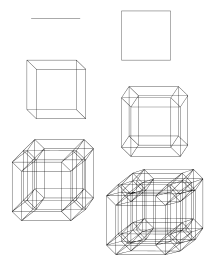
\includegraphics[width=0.3\textwidth]{\subfix{../images/k-cell.png}}\par
  k-cell
\end{figure}

\begin{definition}
  Let $X$ be a metirc space. All points and sets mentioned below are understood to be elements and subsets of $X$.
  \begin{enumerate}[label=(\alph*)]
    \item A \textit{neighborhood} of $p$ is a set $N_r(p)$ consisting of all $q$ such that $d(p,q)<r$, for some $r>0$.
          The number $r$ is called the \textit{radius} of $N_r(p)$.
    \item A point $p$ is a \textit{limit point} of the set $E$ if \textit{every} neighborhood of $p$ contains a point
          $q \ne p$ such that $q \in E$.
    \item If $p \in E$ and $p$ is not a limit point of $E$, then $p$ is called an \textit{isolated point} of $E$.
    \item $E$ is \textit{closed} if every limit point of $E$ is a point of $E$.
    \item A point $p$ is an \textit{interior} point of $E$ if there is a neighborhood $N$ of $p$ such that $N \subset E$.
    \item $E$ is \textit{open} if every point of $E$ is an interior point of $E$.
    \item The \textit{complement} of E (denoted by $E^c$) is the set of all points $p \in X$ such that $p \notin E$.
    \item $E$ is \textit{perfect} if $E$ is closed and if every point of $E$ is a limit point of $E$.
    \item $E$ is \textit{bounded} if there is a real number $M$ and a point $q \in X$ such that $d(p,q)<M$ for all
          $p \in E$.
    \item $E$ is \textit{dense} in $X$ if every point of $X$ is a limit point of $E$, or a point of $E$ (or both).
  \end{enumerate}
\end{definition}

注意 $R^1$ 的邻域为线段,而 $R^2$ 的邻域是圆圈的内点们。

\begin{anote}
  \begin{itemize}
    \item 邻域 neighborhood:到 $p$ 点距离小于 $r$ 的集合($r>0$);
    \item 极限点 limit point:所有邻域存在一个与 $p$ 不同的点,无论半径多小(例如一维空间的开闭区间 $(a,b],\ a<b, \ a,b \in R$
          的 $a,b$ 点皆为极限点,$a$ 虽然不属于 $(a,b]$,但是其右侧总是会有一个点 $p$ 使得 $p-a>0$,$b$ 同理。二维空间集合的
          边间点亦是如此,以此类推所有的边界点皆为极限点);
    \item 孤立点 isolated point:例如 $S = \{0\} \cup [1,2]$ 的 0 点为孤立点;
    \item 闭 closed:如果所有极限点都属于 $E$,那么 $E$ 为闭(例如一维空间 $S=[a,b],\ a<b, \ a,b \in R$,$S$ 为 closed。
          特例:在孤立点构成的度量空间中,任何子集都是即开又闭);
    \item 内点 interior point:用一维空间解释就是 $S=[a,b],\ a<b,\ a,b \in R$ 且 $p \in (a,b)$,那么 $p$ 为 $S$ 的内点;
    \item 开 open:如果 $E$ 中任意一点都是内点,$E$ 为开;
    \item 补集 complement:$\forall p \in X$ 且 $\forall p \notin E$ 那么 $X$ 为 $E$ 补集;
    \item 完全 perfect:一个闭集合中每一个点都是它的极限点,那么该集合为完全;
    \item 有界的 bounded:如果集合中任意一点都在某个 $r$ 为实数的邻域内,那么该集合为有界的;
    \item 稠密 dense:$X$ 中任意一点都是 $E$ 的一个极限点或者 $E$ 中的一点(例如有理数在实数上稠密)。
  \end{itemize}
\end{anote}

\begin{theorem}
  Every neighborhood is an open set.
\end{theorem}

\begin{proof}
  考虑一个邻域 $E = N_r(p)$,并令 $q$ 为 $E$ 的任意一点。那么则有一个正实数 $h$ 满足
  \[d(p,q)=r-h.\]
  对于所有满足 $d(q,s)<h$ 的点 $s$,有
  \[d(p,s) \le d(p,q) + d(q,s) < r - h + h = r,\]
  使得 $s \in E$。因此 $q$ 是 $E$ 的一个内点。
\end{proof}

\begin{theorem}
  If $p$ is a limit point of a set $E$, then every neighborhood of $p$ contains infinitely many points of $E$.
\end{theorem}

\begin{proof}
  假设 $p$ 有一个邻域 $N$,其仅包含了有限点的 $E$。令 $q_1,\dots,q_n$ 为 $N \cap E$ 的这些点,它们有别与点 $p$,且令
  \[r = \min\limits_{1 \le m \le n} d(p,q_m)\]
  (我们使用这个记号来表示最小的 $d(p,q_1),\dots,d(p,q_n)$)。一个有限集的最小值很明显是正数,因此 $r>0$。

  邻域 $N_r(p)$ 包含了除了点 $q$ 的 $E$ 即 $q \ne p$,使得 $p$ 不是 $E$ 的一个极限点。这与定理相悖。
\end{proof}

\begin{corollary}
  A finite point set has no limit points.
\end{corollary}

WIP

\subsection*{Compact Sets}

WIP

\subsection*{Perfect Sets}

WIP

\subsection*{Connected Sets}

WIP

\end{document}
